% SVN info for this file
\svnidlong
{$HeadURL$}
{$LastChangedDate$}
{$LastChangedRevision$}
{$LastChangedBy$}
% BRUTTISSIMO PUN E CHE NON È POLITICAMENTE CORRETTA; un volt m'ampere d'aver vist un'ohm che s'incoulomb un'altr'ohm. Ah Joule!
% Metalmeccanico e parrucchiere in un turbine di sesso e politica
\chapter{Campi elettrici e magnetici variabili nel tempo e le equazioni di Maxwell}
\labelChapter{elettromagnetismoTempo}

\begin{introduction}
	‘‘Sono un esperto di Elettricità. Mio padre ha occupato la cattedra di Elettricità Applicata nella	prigione di stato.''
	\begin{flushright}
		\textscsl{W.C. Fields,} perito (R.I.P.) elettrotecnico e famoso esperto nel campo.
	\end{flushright}
\end{introduction}
\lettrine[findent=1pt, nindent=0pt]{N}{el} capitolo precedente abbiamo finalmente raggiunto un primo, grande risultato: abbiamo enunciato le quattro \textit{equazioni di Maxwell}, le leggi fondamentali che descrivono i fenomeni elettrici e magnetici statici - ossia \textit{costanti nel tempo}:
\begin{align*}
	\div{\vba{E}}=\frac{\rho}{\epsilon_0}&&\curl{\vba{E}}=0\\
	\div{\vba{B}}=0&&\curl{\vba{B}}=\mu_0\vba{j}
\end{align*}
Possiamo suddividere le equazioni in due coppie: due di queste leggi riguardando il campo elettrico $\vba{E}$, mentre le altre due il campo magnetico di induzione $\vba{B}$. All'apparenza queste due coppie sono completamente separate e potrebbero essere risolte senza che una soluzione influenzi l'altra.\\
Tuttavia, già in questa situazione statica non sono completamente indipendenti: le cariche elettriche (nelle equazioni di Maxwell rappresentante dalla densità di carica $\rho$) sono le sorgenti di $\vba{E}$, ma quando sono in movimento danno luogo ad una densità di corrente e quindi diventano \textit{anche} sorgente di $\vba{B}$... ma essere o meno in moto è un fatto \textit{relativo} che dipende dal sistema di riferimento! Un campo elettrico per un sistema di riferimento può apparire come campo magnetico in un altro sistema (o viceversa). È intuibile che $\vba{E}$ e $\vba{B}$ devono essere la manifestazione di un unico ente fisico, il \textit{campo elettromagnetico}. Oltre modo, non possiamo escludere che tale ente dipenda anche dal tempo.\\
Inizieremo a raccogliere prove di questa nostra intuizione studiando i fenomeni elettrici e magnetici \textit{non stazionari}. In questo capitolo partiremo da osservazioni sperimentali per formulare la \textbf{legge di induzione di Faraday} e le sue applicazioni - autoflusso, \textbf{induttanza}, induttori e \textbf{circuiti RL}. Successivamente, parleremo delle correzioni da apporre alla \textbf{legge della circuitazione di Ampère} e la loro interpretazione fisica come \textbf{corrente di spostamento}, concludendo finalmente il principale obiettivo intrapreso all'inizio di questo testo: formulare le \textbf{equazioni di Maxwell nel vuoto}.

\section{Legge di Faraday-Neumann-Lenz}
Le osservazioni sperimentali sul fenomeno dell'induzione elettromagnetica di \textbf{Michael Faraday} (1791-1867) in Inghilterra e, separatamente, di \textbf{Joseph Henry} (1887 - 1915) in America misero in evidenza che un campo magnetico \textit{variabile nel tempo} genera un campo elettrico \textit{non conservativo}. Rivediamo assieme alcuni di questi esperimenti.
\begin{itemize}
	\item \textbf{Esperimento \#1.} Consideriamo una spira collegata ad un circuito - che \textit{non} presenta alcun generatore - dotato di un \textit{amperometro}, cioè di un \textit{misuratore di corrente}. \textit{Avvicinando} un magnete all'interno della spira si \textit{produce} una corrente elettrica.
\begin{center}
	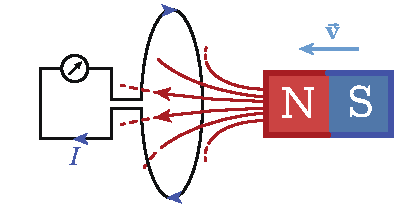
\includegraphics[width=0.35\textwidth]{images/chp10/chp10esperimento1a.pdf}
\end{center}
	Se \textit{allontaniamo} lo stesso magnete alla stessa velocità con cui l'abbiamo avvinato, notiamo ch la corrente che circola ha \textit{cambiato verso di percorrenza}.
\begin{center}
	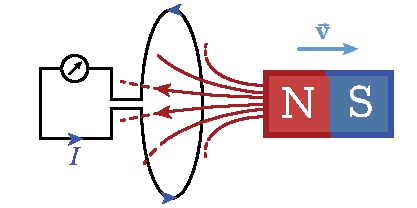
\includegraphics[width=0.35\textwidth]{images/chp10/chp10esperimento1b.pdf}
\end{center}
	\item \textbf{Esperimento \#2.} Consideriamo una spira a cui colleghiamo un generatore di \fem In quanto percorsa da corrente, la spira produce un campo magnetico. Se avviciniamo tale apparato ad un altra spira scarica e collegata ad un amperometro, lo strumento della seconda spira inizia a misurare una corrente. Se la allontaniamo, la corrente nella seconda spira girerà in senso opposto.\\
	\begin{minipage}{0.49\textwidth}
		\begin{center}
			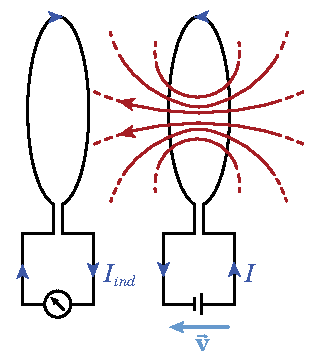
\includegraphics[width=0.6\textwidth]{images/chp10/chp10esperimento2a.pdf}
		\end{center}
	\end{minipage}
	\begin{minipage}{0.49\textwidth}
		\begin{center}
			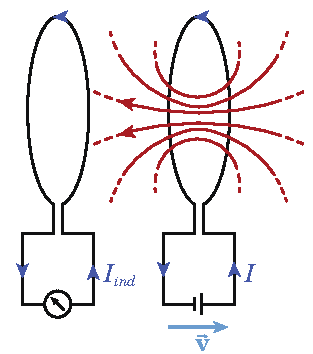
\includegraphics[width=0.6\textwidth]{images/chp10/chp10esperimento2b.pdf}
		\end{center}
	\end{minipage}\\
	\item \textbf{Esperimento \#3 (esperimento di Faraday)}. Consideriamo un solenoide con al suo interno un'anima di ferro - un cilindretto metallico; il solenoide è collegato ad un circuito dotato di interruttore e generatore di \fem Quando l'interruttore è aperto non circola corrente e dunque non si ha alcun campo.
	\begin{center}
		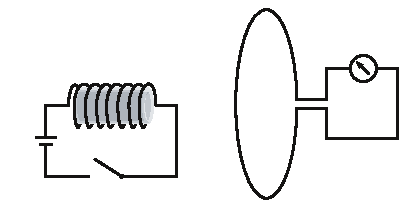
\includegraphics[width=0.35\textwidth]{images/chp10/chp10esperimento3a.pdf}
	\end{center}
	Poniamo ora la solita spira scarica collegata ad un amperometro. Alla chiusura dell'interruttore il solenoide, essendo percorso da corrente, genera un campo magnetico crescente fino a stabilizzarsi. Al contempo, nella spira inizialmente scarica lo strumento segna per qualche istante un passaggio di corrente in una certa direzione, per poi sparire.\\
		\begin{minipage}{0.49\textwidth}
			\begin{center}
				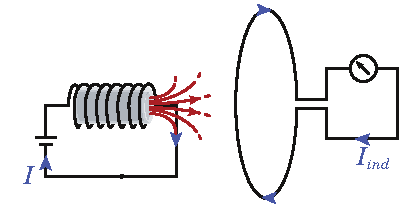
\includegraphics[width=0.6\textwidth]{images/chp10/chp10esperimento3b.pdf}
			\end{center}
		\end{minipage}
		\begin{minipage}{0.49\textwidth}
			\begin{center}
				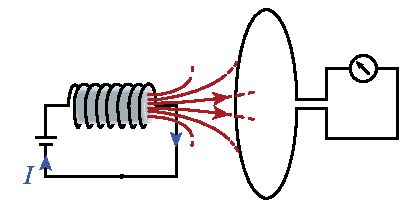
\includegraphics[width=0.6\textwidth]{images/chp10/chp10esperimento3c.pdf}
			\end{center}
		\end{minipage}
	Appena riapriamo l'interruttore la corrente nel solenoide diminuisce e con esso il campo magnetico; allo stesso tempo, osserviamo una corrente nella seconda spira diretta nella direzione opposta a quella precedente. Quando il campo magnetico si spegne del tutto, non osserviamo più la corrente indotta.
	\begin{center}
		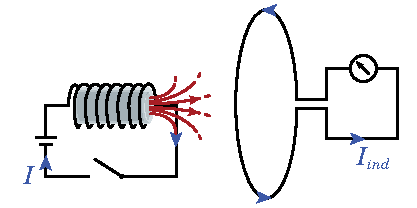
\includegraphics[width=0.35\textwidth]{images/chp10/chp10esperimento3d.pdf}
	\end{center}
\end{itemize}
Da questi esperimenti\footnote{E tante altre varianti di essi che non vedremo perché questo è un Manualozzo\texttrademark\ di Fisica, non un testo monografico su Faraday e i suoi passatempi perversi.} possiamo ricavare diverse informazioni importanti:
\begin{enumerate}[label=\alph*)]\label{osservazioniFaraday} %t
	\item \textit{Spostare una sorgente} di un campo magnetico nei pressi di una spira genera una \fem
	\item Il moto della sorgente rispetto alla spira influenza il \textit{verso di percorrenza} della corrente lungo di essa.
	\item \textit{Spostare una spira} nei pressi di un campo magnetico stazionario genera una \fem in quel circuito.
	\item \textit{Deformare una spira} nei pressi di un campo magnetico stazionario genera una \fem in quel circuito.
	\item Come viene mossa o deformata la spira influenza il \textit{verso di percorrenza} della corrente lungo di essa.
	\item È sufficiente che ci sia una \textit{variazione temporale di un campo magnetico} fisso per causare una \fem in una spira anch'essa fissa.
	\item Come varia temporalmente il campo magnetico fisso influenza il verso di percorrenza della corrente lungo di essa.
	\item Se il campo magnetico non varia più nel tempo - perché si è stabilizzato oppure perché non c'è più la sorgente del campo - non circola più corrente nella spira.
\end{enumerate}
La forza elettromotrice dipende dunque da diversi fattori: la \textit{posizione} e l'\textit{intensità} del campo magnetico, la \textit{posizione} e la \textit{forma della spira}, ma soprattutto la \textit{variazione nel tempo} di tutti questi elementi qui citati.
% Maxwell lavorando a livello teorico sulla consistenza delle equazioni ha scoperto che un campo elettrico e variabile nel tempo produce un campo magnetico.\\
Il concetto matematico che permette di descrivere contemporaneamente un campo vettoriale e come si relaziona con una superficie è quello del \textit{flusso}; per tenere conto degli effetti temporali si deduce che la forza elettromotrice deve dipendere dalla \textit{derivata temporale} dal flusso del $\vba{B}$. Abbiamo descritto quella che è nota come \textbf{legge di Faraday}.
\begin{theorema}[Legge dell'induzione di Faraday o legge di Faraday-Neumann legge di Faraday-Neumann-Lenz]\index{legge!dell'induzione di Faraday}\index{legge!di Faraday-Neumann}\index{legge!di Faraday-Neumann-Lenz}
	Dato un campo magnetico $\vba{B}$ e un circuito chiuso $\gamma$, dove $\gamma$ è il bordo di una superficie $\Sigma$ arbitraria, la \textbf{forza elettromotrice indotta} da $\vba{B}$ in $\gamma$ è pari a
	\begin{equation}
		\mathcal{E}_i=-\dv{\Phi_\Sigma (\vba B)}{t}
	\end{equation}
\end{theorema}
Grazie alla \textit{legge di Ohm} è immediato ricavare la corrente elettrica prodotta dalla \fem indotta per un circuito con resistenza $R$:
\begin{equation}
	I=-\frac{1}{R}\dv{\Phi_\Sigma(\vba B)}{t}
\end{equation}

\begin{observe} %https://en.wikipedia.org/wiki/Electromotive_force
	Nel \autoref{chap:correnteElettrica}, sezione \ref{femxesteso}, abbiamo descritto come la forza elettromotrice è prodotta da un campo elettrico \textit{non} conservativo. Nel caso particolare dell'\textit{induzione magnetica}, il campo magnetico \textit{causa} lungo circuito un campo elettromotore indotto $\vba{E}_i$, non necessariamente localizzato in alcun tratto specifico; l'espressione della forza elettromotrice sarà dunque
	\begin{equation*}
		\mathcal{E}_i=\oint\vba{E}_i\vdot d\vba{s}
	\end{equation*}
	È immediato poter riscrivere la legge di Faraday come
	\begin{equation}
		\oint \vba E_i\vdot d\vba s =-\dv{\Phi_{\Sigma}(\vba B)}{t}		
	\end{equation}
\end{observe}
\paragraph{Legge di Lenz}
Nella legge di induzione troviamo, curiosamente, un meno. Non è un refuso tipografico, ma è una considerazione di natura qualitativa che va sotto il nome di \textbf{legge di Lenz}.
\begin{corollaryqed}[Legge di Lenz]\index{legge!di Lenz}
	La forza elettromotrice indotta - e di conseguenza la corrente indotta - è tale da \textit{opporsi} alla causa che l'ha generata e da esercitare una forza meccanica che si oppone al moto. 
\end{corollaryqed}
\begin{observe}
	Torniamo all'esperimento \# 2 visto precedentemente. La spira percorsa da corrente $I$ viene avvicinata alla spira scarica, crea una variazione nel flusso del campo magnetico $\vba{B}$ generato da $I$. Nella spira scarica inizia a circolare una corrente $I_{ind}$, ma nella direzione opposta a $I$, in modo da generare a sua volta un campo magnetico opposto $\vba{B}_{ind}$ per opporsi a $\vba{B}$.
	\begin{center}
		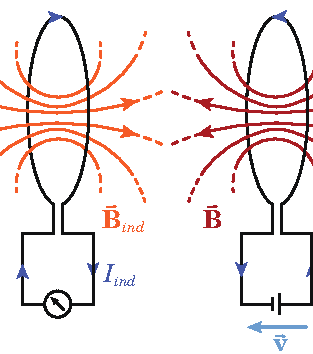
\includegraphics[width=0.35\textwidth]{images/chp10/chp10esperimento2aoss.pdf}
	\end{center}
\end{observe}
Per citare il fisico-divulgatore americano \textbf{D.J. Griffiths} (1942), la legge di Lenz si può sintetizzare come ‘‘\textit{la Natura aberra un cambio di flusso}''.
\paragraph{Com'è bello variar un flusso da Faraday in giù}
%TODO: you've just got Carràrolled
Abbiamo capito che la $\fem$ indotta $\mathcal{E}$ è data da una variazione \textit{temporale} di flusso. Ma come possiamo farlo? Noto che il flusso è dato da
\begin{equation*}
	\Phi_\Sigma(\vba B)=\int_\Sigma \vba B\vdot \vbh{u}_n d\Sigma	
\end{equation*}
e ricordando le osservazioni di pag. \pageref{osservazioniFaraday}, possiamo cambiarlo in diversi modi.
\begin{itemize}
	\item \textit{Spostando rigidamente} il circuito in un campo magnetico, purché non sia soltanto traslatorio in un campo uniforme; infatti, in tal caso non varia mai l'angolo tra la normale del circuito e il campo magnetico, il cui coseno è $\vba{B}\vdot \vbh{u}_n$, e dunque non varia neanche il flusso.\\
	Invece, se il campo magnetico \textit{non} è uniforme o se il moto è \textit{rotatorio}, allora il flusso varia: nel primo caso varia al variare della posizione del circuito nello spazio, mentre nel secondo caso cambia perché cambia l'orientazione del circuito rispetto al campo magnetico.
	\item \textit{Deformando la forma} del circuito nel tempo. Per il \textit{teorema di Stokes}, il flusso del campo magnetico (uniforme o no) dipende solo dal bordo e non da quale superficie $\Sigma$ si sceglie per calcolarlo, dunque cambiare la forma del circuito cambia la necessariamente le potenziali superfici $\Sigma$ e dunque anche il flusso. Se consideriamo un circuito piano di area interna $\Sigma$, questo metodo corrisponde a far variare il valore di $\Sigma$ nel tempo.
	\item \textit{Spostando la sorgente del campo magnetico}, mantenedo allo stesso tempo il circuito fisso.
	\item \textit{Muovendo un mezzo ferromagnetico magnetizzato} nel campo magnetico (uniforme o no), mantenendo allo stesso tempo il circuito fisso e le sorgenti fisse. Senza andare nei dettagli ora\footnote{Nelle ‘‘XXX'', a pagina \pageref{ferromagnetico} è possibile trovare maggiori informazioni sui materiali ferromagnetici e le loro proprietà.}, il movimento di tale mezzo ridistribuisce le linee del campo $\vba{B}$..
	\item In assenza di \textit{qualsiasi moto relativo tra circuito e campo}, il varia se varia $\vba B$ (uniforme o no) \textit{nel tempo}. 
\end{itemize}
In realtà la forza elettromotrice prodotta per mezzo di tutti i modi eccetto l'ultima è causata dalla \textit{sola} forza di Lorentz - e quindi già prevista in realtà dalle leggi della magnetostatica. Quello che \textit{non} era previsto è la produzione di corrente da parte di una variazione del campo magnetico $\vba B$ nel tempo.\label{faradayavevaascopertoiltempo}
\paragraph{Dimostrazione della legge di Faraday-Neumann-Lenz: i casi stazionari}
Dimostriamo di seguito la legge di induzione di Faraday nel caso particolare di uno spostamento rigido in un campo magnetico \textit{non necessariamente} uniforme, ma costante nel tempo: vogliamo provare che la \fem indotta è soltanto una conseguenza alla forza di Lorentz.
\begin{demonstration}
%TODO: inserire immagine 17.1
	Immaginiamo di spostare un circuito in un campo magnetico $\vba{B}$ \textit{non uniforme}, ma costante nel tempo. Lo spostamento infinitesimo della spira è
	\begin{equation*}
		d\vba{r}=\dv{\vba{r}}{t}dt=\vba{v}dt
	\end{equation*}
	dove $\vba{v}$ è la velocità di spostamento rigido.	Ciascuna carica libera presente nella spira subisce una forza di Lorentz pari a
	\begin{equation*}
		\vba{F}=e\vba{v}\cross\vba{B}
	\end{equation*}
	Il campo elettrico indotto \textit{non} conservativo su ogni carica è
	\begin{equation*}
		\vba{E}_i=\frac{\vba{F}}{e}=\vba{v}\cross\vba{B}
	\end{equation*}
	e tende a far girare le cariche. La forza elettromotrice nella spira è il lavoro prodotto lungo la spira $\gamma$ per spostare le cariche:
	\begin{align*}
		\mathcal{E}_i&=\Gamma_{\gamma}(\vba{E}_i)=\oint_{\gamma} \vba{E}_i\vdot d\vba{s}=\oint_{\gamma} \left(\vba{v}\vdot \vba{B}\right)\vdot d\vba{s}=\oint_{\gamma} \left(d\vba{s}\cross\vba{v}\right)\vdot \vba{B} = \oint_{\gamma} \left(d\vba{s}\cross\dv{\vba{r}}{t}\right)\vdot \vba{B}=\\
		&=\dv{t} \oint_{\gamma}\left(d\vba{s}\cross d\vba{r}\right)\vdot \vba{B}\squarequal
	\end{align*}
	Lo spostamento infinitesimo del circuito individua un cilindro \textit{sbilenco}: il lato è individuato da $d\vba{r}$, mentre i bordi delle basi sono il circuito $\gamma$ e $\gamma$ stesso, preso dopo lo spostamento infinitesimo. Osserviamo che il prodotto vettoriale $d\vba{s}\cross d\vba{r}$ è ortogonale alla superficie laterale ed è in modulo l'elemento di area:
	\begin{equation*}
		d\vba s\cross d\vba r=d\Sigma_{\mathcal{l}}\vbh u_n
	\end{equation*}
	%Di conseguenza,
	%\begin{equation*}
	%	\oint_{\gamma} d\vba s\cross d\vba r = \Sigma_{\mathcal{l}}
	%\end{equation*}=$
	Allora
	\begin{equation*}
		\squarequal \dv{t} \oint_{\gamma}\left(d\Sigma_{\mathcal{l}}\vbh{u}_n\right)\vdot \vba{B}=\dv{t} \oint_{\gamma}\vba{B} \vdot \vbh{u}_nd\Sigma_{\mathcal{l}}=\dv{t}\Phi_{\Sigma_{\mathcal{l}}}(\vba{B})
	\end{equation*}
	Abbiamo trovato che la forza elettromotrice è la variazione temporale del flusso \textit{tagliato}, ossia del flusso tramite la superficie laterale di questo cilindro. Se definiamo
	\begin{equation*}
		\dv{\Phi_{\Sigma}}{t}\coloneqq\lim_{\Delta t\to 0}\frac{\Phi_{\Sigma_2}(\vba{B})-\Phi_{\Sigma_1}(\vba{B})}{\Delta t}
	\end{equation*}
	dove
	\begin{itemize}
		\item $\Sigma_1$ è una superficie con bordo il circuito $\gamma$ \textit{prima} dello spostamento.
		\item $\Sigma_2$  è una superficie con bordo il circuito $\gamma$ \textit{dopo} lo spostamento.
	\end{itemize}
	Poiché il cilindro è una superficie chiusa, per la legge di Gauss per il magnetismo
	\begin{equation*}
		0=\Phi_{\Sigma}(\vba{B})=\Phi_{\Sigma_2}(\vba{B})-\Phi_{\Sigma_1}(\vba{B})+\Phi_{\Sigma_{\mathcal{l}}}(\vba{B})
	\end{equation*}
	Esplicitiamo rispetto al flusso tagliato e dividiamo per l'intervallo di tempo $\Delta t$:
	\begin{equation*}
		\frac{1}{\Delta t}\Phi_{\Sigma_{\mathcal{l}}}(\vba{B})=\frac{\Phi_{\Sigma_2}(\vba{B})-\Phi_{\Sigma_1}(\vba{B})}{\Delta t}
	\end{equation*}
	Passando al limite, si ha
	\begin{equation*}
		\mathcal{E}_i=-\dv{t}\Phi_{\Sigma}(\vba{B})
	\end{equation*}
	dove $\Sigma$ è una superficie arbitraria che finisce sul circuito.
\end{demonstration}
In modi analoghi possiamo provare che la \fem indotta dalla variazione di forma e di angolo sono conseguenze soltanto della forza di Lorentz.
\section{Legge di induzione di Faraday}
Abbiamo capito che il fatto che la forza elettromotrice prodotta da un campo magnetico \textit{variabile nel tempo} non è prevedibile dalle leggi di Maxwell già note. Per poter descrivere i fenomeni dipendenti dal tempo dobbiamo necessariamente \textit{correggerle}; fra le equazione di Maxwell che possiamo correggere, la prima è proprio quella che avevamo chiamato senza un ben preciso motivo \textit{legge di induzione di Faraday}:
\begin{equation*}
	\curl{\vba{E}}=0
\end{equation*}
Se il nome vi è \textit{familiare}, è proprio perché è la \textit{stessa} legge di cui abbiamo parlato fino ad ora! La formulazione corretta di questa legge la possiamo dunque ricavare dalla legge (sperimentale) di Faraday.
\begin{theorema}[Legge di induzione di Faraday]\index{legge!di induzione di Faraday}
	Dato il campo elettrico $\vba{E}$ e quello magnetico $\vba{B}$, presa una superficie $\Sigma$ con bordo $\gamma=\partial \Sigma$ si hanno le seguenti relazioni:
	\begin{itemize}
		\item \textbf{Forma integrale:}
		\begin{equation}
			\Gamma_{\gamma}(\vba{E})=\oint_{\partial \Sigma} \vba{E}\vdot d\vba{s}=-\dv{t}\int_{\Sigma}\vba{B}\vdot\vbh{u}_nd\Sigma=-\int_{\Sigma}\pdv{\vba{B}}{t}\vdot\vbh{u}_nd\Sigma\label{LeggeFaradayIntegrale}
		\end{equation}
		\item \textbf{Forma differenziale:}
		\begin{equation}
			\curl{\vba{E}}=-\pdv{\vba{B}}{t}\label{LeggeFaradayDifferenziale}
		\end{equation}
	\end{itemize}
	In altri termini, un campo magnetico variabile nel tempo è accompagnato da un campo elettrico \textit{non} conservativo variante nello spazio e potenzialmente anche nel tempo, e viceversa.
\end{theorema}
\begin{demonstration}
	Partiamo dalla legge di Faraday nota supponendo che $\vba{B}$ sia dipendente anche dal tempo 
	\begin{equation*}
		\mathcal{E}_i=-\dv{t}\Phi_\Sigma(\vba{B})\implies \oint_{\partial \Sigma} \vba{E}\vdot d\vba{s}=-\dv{t}\int_{\Sigma}\vba{B}\vdot \vbh{u}_nd\Sigma
	\end{equation*}
	Qui abbiamo considerato il campo elettrico \textit{totale} lungo il circuito, cioè la somma del campo elettrostatico $\vba{E}_s$ e di quello elettromotore \textit{non} conservativo $\vba{E}_i$ - ricordiamo che il contributo lungo il circuito chiuso di $\vba{E}_s$ è nullo. Ora, portando dentro all'integrale superficiale la derivata temporale e applicando il teorema del rotore all'integrale curvilineo otteniamo la \textit{forma integrale} della legge di induzione magnetica di Faraday:
	\begin{equation*}
		\int_{\Sigma}\left(\curl{\vba{E}}\right)\vdot\vbh{u}_nd\Sigma=-\int_{\Sigma}\pdv{\vba{B}}{t}\vdot\vbh{u}_nd\Sigma
	\end{equation*}
	Poiché la relazione rimane invariata qualunque siano i campi $\vba{E}$ e $\vba{B}$ e qualunque sia la superficie $\Sigma$, vale l'identità tra le integrande. Abbiamo ottenuto così la \textit{forma differenziale} della legge di induzione magnetica di Faraday:
	\begin{equation*}
		\curl{\vba{E}}=-\pdv{\vba{B}}{t}\qedhere
	\end{equation*}
\end{demonstration}
\paragraph{Requiem per il potenziale elettrostatico}
La conseguenza più grande di questa equazione di Maxwell corretta è che il \textit{campo elettrico non è più conservativo} - almeno in generale. Ci chiediamo però se sia comunque possibile esprimerlo in termini di opportuni campi potenziali.\\
Dalla \textit{legge di Gauss per il magnetismo} sappiamo che il campo magnetico è \textit{solenoidale} e quindi esiste localmente un campo potenziale vettoriale $\vba{A}$ tale per cui
\begin{equation*}
	\vba{B}=\curl{\vba{A}}
\end{equation*}
Per la legge di induzione di Maxwell si ha
\begin{equation*}
	\curl{\vba{E}}=-\pdv{\vba{B}}{t}=-\pdv{t}\left(\curl{\vba{A}}\right)\implies \curl\left(\vba{E}+\pdv{\vba{A}}{t}\right)=0
\end{equation*}
Osserviamo che quest'ultima quantità, essendo irrotazionale e quindi conservativa, ammette un campo potenziale scalare $V$ tale che 
\begin{equation*}
	\vba{E}+\pdv{\vba{A}}{t}=-\grad{V}
\end{equation*}
Il campo elettrico è esprimibile quindi come
\begin{equation}
	\vba{E}=-\pdv{\vba{A}}{t}-\grad{V}
\end{equation}
Come si può notare, se siamo nel \textit{caso stazionario} e il campo magnetico $\vba{B}$ \textit{non} varia nel tempo, allora anche $\vba{A}$ è costante temporalmente e quindi si ritorna al caso del campo elettrico \textit{conservativo} - il fu campo \textit{elettrostatico}.
\section{Autoflusso, autoinduzione e induttanza}
Sappiamo che una spira $\gamma$ percorsa da una corrente di intensità $I$ genera un campo magnetico dato dalle legge di Biot-Savart:
\begin{equation*}
	\vba{B}=\frac{\mu_0 I}{4\pi}\oint_{\gamma}\frac{d\vba{s}\cross\vbh{u}_{r}}{r^2}
\end{equation*}
Tale campo produce un flusso \textit{non} nullo attraverso la superficie stessa, detto \textbf{autoflusso}:
\begin{equation}
	\Phi_{\Sigma}(\vba{B})=\int_{\Sigma}\vba{B}\vdot\vbh{u}_nd\Sigma=\frac{\mu_0 I}{4\pi}\int_{\Sigma}\vba\oint_{\gamma}\frac{\left(d\vba{s}\cross\vbh{u}_{r}\right)\vdot \vbh{u}_n}{r^2}d\Sigma
\end{equation}
Dalla legge di Faraday-Neumann-Lenz sappiamo inoltre che nella spira si genererà una \fem $\mathcal{E}_i$ e dunque un'altra corrente $I'$, il cui verso per la legge di Lenz è tale da opporsi al cambio di corrente; in particolare, la corrente $I'$ percorre la corrente nel verso opposto a $I$. Questo fenomeno prende il nome di \textbf{autoinduttanza}\index{autoinduttanza}:
\begin{equation*}
	\mathcal{E}_i=-\dv{t}\Phi_{\Sigma}(\vba{B})=-\dv{t}\frac{\mu_0 I}{4\pi}\int_{\Sigma}\vba\oint_{\gamma}\frac{\left(d\vba{s}\cross\vbh{u}_{r}\right)\vdot \vbh{u}_n}{r^2}d\Sigma
\end{equation*} %TODO: se la spira si deforma è costante?
Osserviamo che il doppio integrale superficiale-curvilineo dipende esclusivamente dalla \textit{geometria} della spira e rimane costante nel tempo. Come abbiamo fatto per il condensatore, possiamo definire una quantità \textit{caratteristica} dei circuiti chiusi che quantifica sia l'informazione geometrica della spira sia, dal punto di vista della legge di Faraday, quella relativa all'opposizione al cambiamento di corrente. 
\begin{define}[Induttanza]
	L'\textbf{induttanza}\index{induttanza} di una spira $\gamma$ è la tendenza della spira ad opporsi ad un cambiamento nella corrente che scorre in esso. Matematicamente, dipende solo dalla natura geometrica del circuito ed è definita da
	\begin{equation}
		L=\frac{\mu_0}{4\pi}\int_{\Sigma}\vba\oint_{\gamma}\frac{\left(d\vba{s}\cross\vbh{u}_{r}\right)\vdot \vbh{u}_n}{r^2}d\Sigma
	\end{equation}
\end{define}
\begin{define}[Autoflusso]
	L'\textbf{autoflusso}\index{autoflusso} di una spira $\gamma$ percorsa da corrente $I$ è il flusso del campo magnetico generato dalla corrente tramite la superficie delimitata dalla spira stessa:
	\begin{equation}
		\Phi_{\Sigma}(\vba{B})=LI
	\end{equation}
	dove $L$ è l'\textit{induttanza} della spira.
\end{define}
La \fem autoindotta si può dunque esprimere come
\begin{equation*}
	\mathcal{E}_i=-\dv{t}\Phi_{\Sigma}(\vba{B})=-\dv{t}\left(LI\right)=-L\dv{I}{t}
\end{equation*}
\begin{equation}
	\mathcal{E}_i=-L\dv{I}{t}
\end{equation}
\begin{example}[Solenoide infinito]
	Supponiamo di avere un \textit{solenoide infinito}, che nella pratica è un solenoide di lunghezza $d$ molto maggiore del suo raggio $R$ in modo da escludere qualunque effetto di bordo. Il campo magnetico è, in modulo,
	\begin{equation*}
		B=\mu_0 I n
	\end{equation*}
	con $n$ la densità lineare di spire. Se nel solenoide ci sono $N$ spire, ò'autoflusso è dato dalla somma degli autoflussi delle singole spire:
	\begin{equation}
		\Phi_{\Sigma}(\vba{B})=\Sigma B N=\pi R^2 \cdot \mu_0 I n \cdot nd=\mu_0 I n^2\Sigma d
	\end{equation}
	L'induttanza è quindi
	\begin{equation}
		L=\mu_0 n^2\Sigma d
	\end{equation}
	dove $\Sigma$ è l'area di una spira del solenoide.
\end{example}
\paragraph{Unità di misura}
\begin{units}~\\
	\textbf{\textsc{Induttanza:}} henry ($\unit{\henry}$) o weber su ampere  ($\unit[per-mode = fraction]{\weber\per\ampere}$) o volt per secondo su ampere ($\unit[per-mode = fraction]{\volt\second\per\ampere}$) o ohm per secondo ($\unit[per-mode = fraction]{\ohm\second}$).\\
	\textit{Dimensioni:} $[L]=\frac{\left[\Phi_{\Sigma}(\vba{B})\right]}{\left[I\right]}=\mathsf{M} \mathsf{L}^2 \mathsf{T}^{-2} \mathsf{I}^{-2}$.
\end{units}
\section{Circuiti RL}
Torniamo in ambito elettrotecnico. Per poter aggiungere dell'induttanza ad un circuito si può far uso di un componente elettrico detto \textbf{induttore}.
\begin{define}[Induttore]
	Un \textbf{induttore}\index{induttore} è un componente elettrico che implementa gli effetti di un induttanza all'interno di un circuito, in modo da aumentare il flusso magnetico.
	\begin{center}
		\begin{tikzpicture}[voltage dir=RP]
			\draw (-0.5,0) to [L=$L$] (1.5,0);
		\end{tikzpicture}
	\end{center}
\end{define}
\begin{example}
	Un classico esempio di induttore e che è l'origine del simbolo elettrico associato agli induttore è il \textit{solenoide}.
\end{example}
\begin{define}[Circuito RL]
	Un \textbf{circuito RL}\index{circuito!RL} è un circuito che presenta solo \textit{resistori} e \textit{induttori}.
	\begin{center}		
		\begin{tikzpicture}[voltage dir=RP]
			\draw (0,0) to [battery1, v>=$\mathcal{E}$] (0,2.5)
			to [resistor, R=$R$, v=$V_R$] (2.5,2.5)
			to [inductor, L=$L$, v=$\mathcal{E}_i$] (2.5,0)
			to [switch, label=$t<0$, mirror] (0,0)
			-- (0,0.1);
			\draw (1,0) to[short, *-] (1,0);
		\end{tikzpicture}
		\begin{tikzpicture}[voltage dir=RP]
			\draw (0,0) to [battery1, v>=$\mathcal{E}$, i=$I$] (0,2.5)
			to [resistor, R=$R$, v=$V_R$] (2.5,2.5)
			to [inductor, L=$L$, v=$\mathcal{E}_i$] (2.5,0)
			-- (0,0) %to [switch, label=$t>0$, mirror] (0,0)
			%-- (0,0) node [midway, below] (TextNode) {$t>0$}
			-- (0,0.1);
			\draw (1,0) to[short, *-] (1,0);
			\node at (1.25,-0.5) {$t>0$};
			\node at (1.25,-0.6) {$ $};
		\end{tikzpicture}
	\end{center}
\end{define}
Consideriamo il caso semplice di un circuito RL, dotato di un interruttore inizialmente aperto, con un resistore e un induttore. Al tempo $t=0$ viene chiuso l'interruttore: poiché si verifica la separazione di cariche da parte del generatore di \fem, la corrente può circolare nel circuito e attraversa l'induttore, generando una forza elettromotrice autoindotta
\begin{equation*}
	\mathcal{E}_i=-L\dv{I}{t}
\end{equation*}
che si oppone a quella $\mathcal{E}$ del generatore.
\begin{observe}
	Inizialmente, la corrente passa lentamente attraverso l'induttore: come per la resistenza, l'induttanza funge da \textit{ostacolo} alla corrente.
\end{observe}
Dalla seconda legge di Kirchhoff, fissato come verso di percorrenza quello della corrente $I$, la somma delle \ddp è
\begin{align*}
	\mathcal{E}+\mathcal{E}_i-V_R=0\\
	\mathcal{E}-L\dv{I}{t}-RI=0
\end{align*}
Risolviamo questa equazione differenziale per descrivere la corrente $I=I(t)$ che attraversa l'induttore.
\begin{align*}%TODO: fix
	&\dv{I}{t}=\frac{\mathcal{E}-RI}{L}\\ &\int_{0}^{I(t)}\frac{dI}{\mathcal{E}-RI}=\frac{1}{L}\int_{0}^{t}dt\\
	&-\frac{1}{R}\eval{\log{\mathcal{E}-RI}}_{0}^{I(t)}=-\frac{1}{L}\eval{t}_{0}^{t}\\
	&-\frac{1}{R}\log{\frac{\mathcal{E}-RI(t)}{\mathcal{E}}}=\frac{t}{L}\\
	&\mathcal{E}-RI(t)=\mathcal{E}e^{-\frac{Rt}{L}}
\end{align*}
\begin{equation}
	I(t)=\frac{\mathcal{E}}{R}\left(1-e^{-\frac{Rt}{L}}\right)=\frac{\mathcal{E}}{R}\left(1-e^{-\frac{t}{\tau}}\right)
\end{equation}
%TODO: inserire grafico
L'andamento temporale della corrente è dettato dal \textbf{tempo caratteristico del circuito RL}\index{tempo caratteristico!del circuito RL}:
\begin{equation}
	\tau=\frac{L}{R}
\end{equation}
Essa è una costante dimensionalmente pari ad una quantità temporale e quindi nel SI si misura in secondi:
\begin{equation*}
	\left[\tau\right]=\frac{\left[L\right]}{\left[R\right]}=\mathsf{M} \mathsf{L}^2 \mathsf{T}^{-2} \mathsf{I}^{-2}\cdot \mathsf{M}^{-1} \mathsf{L}^{-2}  \mathsf{T}^3 \mathsf{I}^{2}=\mathsf{T}
\end{equation*}
La corrente dopo un tempo di carica \textit{infinito} è 
\begin{equation}
	I_{\infty}=\frac{\mathcal{E}}{R}
\end{equation}
ossia a regime l'induttanza smette di fatto di opporsi al generatore e il circuito è equivalente ad un circuito resistore classico.\\
Per un \textit{matematico} questa situazione non si potrebbe mai realizzare; invece, per un \textit{fisico} questo si realizza - approssimando, neh! - per un tempo tra $3\tau=3RC$ e $3\tau=3RC$. Infatti, si ha
\begin{align*}
	I(3\tau)&=\frac{\mathcal{E}}{R}\left(1-e^{-\nicefrac{3\Ccancel[red]{\tau}}{\Ccancel[red]{\tau}}}\right)=\num{0.950}\cdot\frac{\mathcal{E}}{R}\\
	I(5\tau)&=\frac{\mathcal{E}}{R}\left(1-e^{-\nicefrac{3\Ccancel[red]{\tau}}{\Ccancel[red]{\tau}}}\right)=\num{0.993}\cdot\frac{\mathcal{E}}{R}
\end{align*}
i quali sono valori \textit{molto} vicini al valore asintotico $I_{\infty}$ e che nella pratica possiamo assimilare ad esso.\\
Per ottenere la \fem autoindotta ci basta derivare $I(t)$ rispetto al tempo:
\begin{equation}
	\mathcal{E}_i=-L\dv{I(t)}{t}=-\mathcal{E}e^{-\frac{Rt}{L}}
\end{equation}
%TODO: inserire grafico
All'inizio $\mathcal{E}_i$ si oppone \textit{fortemente} al cambio di corrente e quindi al passaggio della stessa dato che è pari alla \fem del generatore $\mathcal{E}$; in seguito diminuisce fino a tendere asintoticamente a zero.
\paragraph{Potenze ed energia nel circuito RL}
Come il \textit{condensatore} immagazzinava energia nel \textit{campo elettrico}, l'\textit{induttore} lo immagazzina nel \textit{campo magnetico} generato da esso.\\
Prima di determinare tale energia, parliamo delle potenze in gioco nel circuito. La potenza erogata dal generatore è
\begin{equation}
	P_{\mathcal{E}}(t)=\mathcal{E}I(t)=\frac{\mathcal{E}^2}{R}\left(1-e^{-\frac{Rt}{L}}\right)
\end{equation}
mentre quella dissipata dalla resistenza e quella associata all'induttore sono
\begin{equation}
	P_{R}(t)=RI^2(t)=\frac{\mathcal{E}^2}{R}\left(1-e^{-\frac{Rt}{L}}\right)^2
\end{equation}
\begin{equation}
	P_{L}(t)=\mathcal{E}_iI(t)=-LI(t)\dv{I(t)}{t}=-\frac{\mathcal{E}^2}{R}e^{-\frac{Rt}{L}}\left(1-e^{-\frac{Rt}{L}}\right)
\end{equation}
Si noti che se la \ddp ai capi del generatore è
\begin{equation}
	\mathcal{E}=RI+L\dv{I}{t}
\end{equation}
si ha
\begin{equation*}
	\mathcal{E}(t)I(t)=RI^2(t)+LI\dv{I(t)}{t}\implies P_{\mathcal{E}}(t)=P_R(t)+P_L(t)
\end{equation*}
Sul lungo termine, l'energia prodotta dall'induttore complessivamente è
\begin{equation*}
	U_L=\int_0^{+\infty}P_Ldt=\int_0^{+\infty} LI(t)\dv{I(t)}{t}dt=\int_{I(0)}^{I(+\infty)}
	LIdI=\frac{1}{2}L\eval{I}_{I(0)}^{I(+\infty)}=\frac{1}{2}LI_{\infty}^2
\end{equation*}
\begin{equation}
	U_L=\frac{1}{2}L I_{\infty}^2=\frac{1}{2}L\frac{\mathcal{E}^2}{R^2}
\end{equation}
\begin{examplewt}[Solenoide]
	Se l'induttore è un solenoide, l'induttanza è
	\begin{equation*}
		L=\mu_0 \Sigma n^2 d
	\end{equation*}
	L'energia immagazzinata nel campo magnetico del solenoide è
	\begin{equation}
		U_L=\frac{1}{2}\mu_0\Sigma n^2 d  I^2=\frac{1}{2}\frac{B^2}{\mu_0}\Sigma d
	\end{equation}
\end{examplewt}
Osserviamo come $\Sigma d$ corrisponde al volume $V$ occupato dal campo magnetico all'interno del solenoide. Se definiamo la \textbf{densità di energia magnetica per unità di volume}\index{densità!di energia magnetica}
\begin{equation}\label{DensitàEnergiaMagnetica}
	\mu_{B}=\frac{1}{2}\frac{B^2}{\mu_0}
\end{equation}
l'energia immagazzinata nell'induttore è questa densità moltiplicata per il volume $V$ \textit{occupato} dal campo magnetico. Dal punto
\section{Energia del campo magnetico}
In generale, il campo magnetico immagazzina \textit{sempre} dell'energia nel campo stesso. Tale energia, in un certo volume $V$, è pari a
\begin{equation}
	U=\int_V\mu_BdV=\frac{1}{2\mu_0}\int_V\abs{\vba{B}(r)}^2dV
\end{equation}
dove $\mu_E$ è la densità di energia magnetica, definita come nell'equazione \eqref{DensitàEnergiaMagnetica}.
\paragraph{Confronto tra energia elettrica e magnetica}
\begin{center}
	\begin{tabular}{p{0.49\textwidth}p{0.49\textwidth}}
		\multicolumn{1}{c|}{\textbf{Caso elettrico}} &
		\multicolumn{1}{c}{\textbf{Caso magnetico}} \\ \hline
		\multicolumn{2}{c}{\textbf{Energia in un}}\\
		\multicolumn{1}{c|}{\textbf{conduttore}} &
		\multicolumn{1}{c}{\textbf{induttore}} \\ \hline
		\multicolumn{1}{c|}{$\displaystyle U_C=\frac{q^2}{2C}=\frac{qV}{2}=\frac{CV^2}{2}$} & \multicolumn{1}{c}{$\displaystyle U_L=\frac{LI^2}{2}$}\\ \hline
		\multicolumn{2}{c}{\textbf{Densità di energia}}\\ \hline
		\multicolumn{1}{c|}{$\displaystyle \mu_E=\frac{\epsilon_0}{2}E^2$} & \multicolumn{1}{c}{$\displaystyle \mu_E=\frac{1}{2\mu_0}B^2$}\\ \hline
		\multicolumn{2}{c}{\textbf{Energia in un volume del campo}}\\ 
		\multicolumn{1}{c|}{\textbf{elettrico}} &
		\multicolumn{1}{c}{\textbf{magnetico}} \\ \hline
		\multicolumn{1}{c|}{$\displaystyle U_E=\frac{\epsilon_0}{2}\int_V E^2dV$} & \multicolumn{1}{c}{$\displaystyle U_B=\frac{1}{2\mu_0}\int_V B^2dV$}\\
	\end{tabular}
\end{center}
Nel caso in cui in un certo volume siano presenti sia il campo elettrico, sia il campo magnetico, le densità di energia si sommano punto per punto:
\begin{equation}
	\mu=\frac{1}{2}\left(\epsilon_0E^2+\frac{B^2}{\mu_0}\right)
\end{equation}
L'energia complessiva sarà quindi
\begin{equation}
	U=\frac{1}{2}\int_V \epsilon_0E^2+\frac{B^2}{\mu_0}dV=U_E+U_B
\end{equation}
\section{Legge della circuitazione di Maxwell-Ampère}
Nel \autoref{chap:leggediampere}, sezione \ref{laleggediAmpereèfalsaepretenziosa} a pag. \pageref{laleggediAmpereèfalsaepretenziosa}, abbiamo osservato la \textit{non validità} della legge di Ampère
\begin{align*}
	&\Gamma_{\gamma}(\vba{B})=\oint_{\partial \Sigma} \vba{B}\vdot d\vba{s}=\mu_0\int_{\Sigma}\vba{j}\vdot\vbh{u}_nd\Sigma=\mu_0 I_{int}	&& \left(\text{forma integrale}\right)\\
	&\curl{\vba{B}}=\mu_0\vba{j}	&& \left(\text{forma differenziale}\right)\\
\end{align*}
in \textit{condizioni non stazionarie}. Infatti, applicando la divergenza ad entrambi i membri della forma differenziale della legge ottenevamo che essa era consistente soltanto se la \textit{densità di corrente risultasse solenoidale},
\begin{equation}
	\div{\vba{j}}=0,
\end{equation}
fatto che se la densità di carica varia nel tempo non è più vero sulla base dell'equazione di continuità
\begin{equation*}
	\div{\vba{j}}+\pdv{\rho}{t}=0
\end{equation*}
La correzione di questa legge deve garantire la validità dell'equazione di continuità.
Dalla \textit{legge di Gauss per l'elettricità} sappiamo che
\begin{equation*}
	\div{\vba{E}}=\frac{\rho}{\epsilon_0}\implies \rho=\epsilon_0\div{\vba{E}}
\end{equation*}
Derivando entrambi i membri temporalmente otteniamo
\begin{equation}
	\pdv{\rho}{t}=\epsilon_0\div{\pdv{\vba{E}}{t}}\label{Passo1LeggeAmpere}
\end{equation}
Ora, sostituendo \eqref{Passo1LeggeAmpere} nell'equazione di continuità, vediamo che
\begin{equation}
	\div{\vba{j}}+\epsilon_0\div{\pdv{\vba{E}}{t}}=\div{\left(\vba{j}+\epsilon_0\pdv{\vba{E}}{t}\right)}=0
\end{equation}
Nel caso non stazione, quello che è sempre un vettore \textit{solenoidale} è il vettore
\begin{equation*}
	\vba{j}_{tot}=\vba{j}+\epsilon_0\pdv{\vba{E}}{t}
\end{equation*}
Introduciamo le seguenti definizioni.
\begin{define}[Corrente di spostamento e densità di corrente di spostamento]
	La \textbf{densità di corrente di spostamento}\index{densità!di corrente di spostamento} è la quantità vettoriale
	\begin{equation}
		\vba{j}_s=\epsilon_0\pdv{\vba{E}}{t}
	\end{equation}
	L'intensità di \textbf{corrente di spostamento} è il suo flusso attraverso una superficie $\Sigma$:
	\begin{equation}
		I_S=\int_{\Sigma}\vba{j}_s\vdot \vbh{u}_nd\Sigma=\epsilon_0\int_{\Sigma}\epsilon_0\pdv{\vba{E}}{t}\vdot \vbh{u}_nd\Sigma=\epsilon_0\pdv{\Phi_{\Sigma}(\vba{E})}{t}
	\end{equation}
\end{define}
Dimensionalmente parlando, queste due quantità hanno rispettivamente le stesse dimensioni di una densità di corrente elettrica e un'intensità di corrente elettrica, come i nomi giustamente suggeriscono. Non approfondiamo adesso la spiegazione fisica di \textit{cosa} effettivamente rappresentano   - ma lo faremo tra poco; per ora torniamo alla legge di Ampère.\\
Posta questa nomenclatura, l'idea è di modificare la legge di Ampère sostituendo alla densità di corrente $\vba{j}$ la \textbf{densità totale}
\begin{equation*}
	\vba{j}_{tot}=\vba{j}+\vba{j}_s=\vba{j}+\epsilon_0\pdv{\vba{E}}{t}
\end{equation*}
Otteniamo quindi la
\begin{theorema}[Legge della circuitazione di Maxwell-Ampère]\index{legge!della circuitazione di Maxwell-Ampère}
	Dato il campo elettrico $\vba{E}$ e quello magnetico $\vba{B}$, presa una superficie $\Sigma$ con bordo $\gamma=\partial \Sigma$ si hanno le seguenti relazioni:
	\begin{itemize}
		\item \textbf{Forma integrale:}
		\begin{multline}
			\Gamma_{\gamma}(\vba{B})=\oint_{\partial \Sigma} \vba{B}\vdot d\vba{s}=\mu_0\left(\int_{\Sigma}\vba{j}\vdot\vbh{u}_n d\Sigma+\epsilon_0\dv{t}\int_{\Sigma}\vba{E}\vdot\vbh{u}_nd\Sigma\right)=\\
			=\mu_0 I_{int}+\frac{1}{c^2}\pdv{\Phi_{\Sigma}(\vba{E})}{t}=\mu_0\left(I+I_s\right)\label{LeggeAmpereIntegrale}
		\end{multline}
		\item \textbf{Forma differenziale:}
		\begin{equation}
			\curl{\vba{B}}=\mu_0\left(\vba{j}+\epsilon_0\pdv{\vba{E}}{t}\right)=\mu_0\left(\vba{j}+\vba{j}_s\right)=\mu_0\vba{j}_{tot}\label{LeggeAmpereDifferenziale}\qedhere
		\end{equation}
	\end{itemize}
\end{theorema}
\begin{demonstration}
	Verifichiamo rapidamente che la riformulazione della legge di Ampère è \textit{consistente} con l'equazione di continuità.\\ 
	Applicando la divergenza ad entrambi i membri della \eqref{LeggeAmpereDifferenziale}, si ha
	\begin{equation}
		0=\div{\left(\curl{\vba{B}}\right)}=\Ccancel[red]{\mu_0}\div{\vba{j}}+\Ccancel[red]{\mu_0}\epsilon_0\div{\pdv{\vba{E}}{t}}\label{Passo2DimleggeAmpere} 
	\end{equation}
	Sostituendo la \eqref{Passo1LeggeAmpere}, trovata precedentemente, dentro la \eqref{Passo2DimleggeAmpere} otteniamo l'equazione di continuità come richiesto:
	\begin{equation*}
		\div{\vba{j}}+\pdv{\rho}{t}=0\qedhere
	\end{equation*}
\end{demonstration}
\subsection{Interpretazione fisica della corrente di spostamento}
Oltre ai motivi di \textit{natura matematica} che abbiamo affrontato, la non validità della legge di Ampère e la necessità di introdurre una ‘‘corrente di spostamento'' si può constatare anche dal punto di vista \textit{fisico} in diversi esperimenti, in cui notiamo una \textit{discrepanza} tra i risultati teorici previsti e quelli osservati.

Uno dei più esemplificativi è quello del \textit{processo di carica di un condensatore} per mezzo di un circuito RC, di cui abbiamo parlato nel \autoref{chap:correnteElettrica}, sezione \ref{CircuitiRC}, pag. \pageref{CircuitiRC}.\\
Ricordiamo che, come detto nell'osservazione di pag. \pageref{correntevariabile}, all'\textit{interno} del condensatore \textit{non} ci sono cariche e dunque neanche una \textit{corrente di conduzione}, ma ai capi del condensatore si ha virtualmente la stessa corrente per repulsione delle cariche. Consideriamo ora un cilindro immaginario $\Sigma$ coassiale al filo e calcoliamo l'intensità di corrente tramite esso in due situazioni differenti: 
\begin{itemize}
	\item Se il cilindro $\Sigma$ racchiude al suo interno \textit{entrambe} le armature del condensatore, il flusso netto è nullo. Infatti, a patto di non avere variazioni troppo brusche della carica sulle piastre la densità di carica $\vba{j}$ è la stessa ad entrambi i capi e quindi ‘‘tutto ciò che entra esce''
	\begin{equation*}
		i=\dv{q}{t}=\int_{\Sigma}\vba{j}\vdot\vbh{u}_nd\Sigma=0
	\end{equation*} 
	\item Se il cilindro $\Sigma$ contiene \textit{soltanto una} delle due armature - non è fondamentale quale - il flusso di $\vba{j}$ \textit{non} è nullo perché c'è una carica entrante o uscente la superficie, ma essa non è controbilanciata da altre cariche uscenti o entranti dal resto della superficie, in quanto nello spazio tra le armature \textit{non} passano particelle libere!
\end{itemize}
Nel secondo caso, suddividiamo la superficie $\Sigma$ in due sottosuperfici $\Sigma_i$ di bordo comune $\partial \Sigma$:
\begin{itemize}
	\item $\Sigma_1$ è la base del cilindro, che interseca il filo ma \textit{non} lo spazio in mezzo alle armature.
	\item $\Sigma_2$ è il resto del cilindro, che interseca lo spazio in mezzo alle armature ma \textit{non} il filo.
\end{itemize}
Per la prima superficie $\vba{j}$ lì esiste e quindi l'integrale non è nullo...
\begin{equation*}
	\int_{\Sigma_1}\vba{j}\vdot\vbh{u}_n=I=\dv{q}{t}
\end{equation*}
... d'altro canto la seconda superficie, non incontrando il filo, \textit{non} presenta alcuna corrente e quindi
\begin{equation*}
	\int_{\Sigma_2}\vba{j}\vdot\vbh{u}_n=0
\end{equation*}
Sappiamo inoltre che il filo percorso da corrente genera un campo magnetico $\vba{B}$ e il valore della circuitazione di di esso lungo $\partial \Sigma$ \textit{non} è nullo; per la legge di Ampère nella formulazione elettrostatica ci porterebbe a dire che
\begin{equation*}
	I=\int_{\Sigma_1}\vba{j}\vdot\vbh{u}_n=\oint_{\partial \Sigma}\vba{B}\vdot\vbh{u}_nd=\int_{\Sigma_2}\vba{j}\vdot\vbh{u}_n=0
\end{equation*} 
il che è decisamente assurdo. Inoltre, nel caso considerato $\vba{j}$ non sarebbe solenoidale come previsto invece dalla legge di Ampère.

Sembrerebbe dunque che oltre al campo magnetico dato dal filo percorso da corrente ci sia un \textit{altro} campo magnetico generato da qualcosa interno alle piastre; per la \textit{legge di Biot-Savart}, quel \textit{qualcosa} dovrebbe essere una \textit{corrente}... ma che sappiamo non esistere!\\
Maxwell propone come ipotesi per risolvere questo \textit{impasse} proprio quella di supporre l'esistenza di una corrente \textit{fittizia}
\begin{equation*}
	\vba{j}_s=\epsilon_0\pdv{\vba{E}}{t}
\end{equation*}
e di intensità
\begin{equation*}
	I_S=\epsilon_0\int_{\Sigma}\epsilon_0\pdv{\vba{E}}{t}\vdot \vbh{u}_nd\Sigma
\end{equation*}
che \textit{scorre tra le piastre} nella stessa direzione della corrente di conduzione $\vba{j}$ - come se \textit{spostasse virtualmente} le cariche da una piastra all'altra.
Lungo l'intero circuito (spazio tra le armature comprese) possiamo quindi considerare una \textit{densità di carica totale}
\begin{equation*}
	\vba{j}_{tot}=\vba{j}+\vba{j}_s
\end{equation*}
dove $\vba{j}$ esiste \textit{solo} lungo i fili e $\vba{j}$ esiste \textit{solo} tra le armature del condensatore. Le considerazioni matematiche precedenti ci hanno confermato che, almeno in linea teorica, sostituire nella legge di Ampère a $\vba{j}$ il vettore $\vba{j}_{tot}$ garantisce l'equazione di continuità e di avere una densità di carica (totale) solenoidale.\\
Ripercorriamo il ragionamento precedente con la densità di carica totale, osservando che per la prima superficie $\vba{j}_{tot}=\vba{j}$...
\begin{equation*}
	\int_{\Sigma_1}\vba{j}_{tot}\vdot\vbh{u}_n=\int_{\Sigma_1}\vba{j}\vdot\vbh{u}_n=I=\dv{q}{t}
\end{equation*}
... e per la seconda superficie $\vba{j}_{tot}=\vba{j}_s$, osservando che il campo elettrico generato dalle cariche che stanno sulle armature è diverso da zero:
\begin{equation*}
	\int_{\Sigma_2}\vba{j}_{tot}\vdot\vbh{u}_n=\int_{\Sigma_2}\vba{j}\vdot\vbh{u}_n=\epsilon_0\int_{\Sigma_2}\pdv{\vba{E}}{t}\vdot\vbh{u}_n=I_S
\end{equation*}
Dato che $\vba{j}_{tot}$ è solenoidale, i due flussi ottenuti devono essere uguali.
\begin{equation*}
	I=\int_{\Sigma_1}\vba{j}\vdot\vbh{u}_n=\int_{\Sigma_1}\vba{j}_{tot}\vdot\vbh{u}_n=\oint_{\partial \Sigma}\vba{B}\vdot\vbh{u}_nd=\int_{\Sigma_2}\vba{j}_{tot}\vdot\vbh{u}_n=\int_{\Sigma_2}\vba{j}_{s}\vdot\vbh{u}_n=I_s
\end{equation*}
\begin{equation}
	I=I_s
\end{equation}
La \textit{corrente totale} ha lo stesso valore lungo l'intero circuito: coincide con $I$ nei cavi di collegamento e $I_s$ all'interno del condensatore.
\begin{attention}
	Nonostante il nome suggestivo, con la corrente di spostamento \textit{non avviene alcun moto} fisico di cariche!
\end{attention}
\begin{digression}
	Fra le equazioni di Maxwell, questa è l'\textit{ultima} ad essere stata scoperta. Il contributo al campo magnetico fornito dalla variazione del campo elettrico è molto piccolo a causa del fattore $\nicefrac{1}{c^2}$; per questo motivo, fu ipotizzata \textit{prima} dal punto di vista \textit{teorico} e solo \textit{successivamente}  comprovata \textit{empiricamente}, quando lo sviluppo di strumenti sufficientemente precisi permisero di misurare con certezza tale contributo.
\end{digression}
\section{Equazioni di Maxwell dell'elettromagnetismo classico}
\begin{center}
	\begin{tabular}{p{0.18\textwidth}|c|c}
		%\multicolumn{2}{c}{\textbf{---}} \\\hline  >{\centering}
		\centering{\textbf{Nome}} &
		\textbf{Forma integrale} &
		\begin{tabular}{@{}c@{}} \textbf{Forma} \\ \textbf{differenziale}\end{tabular} \\ \hline
		
		\begin{tabular}[c]{@{}p{0.18\textwidth}@{}}	
			\\[-2mm]\textbf{Legge di Gauss per l'elettricità}\\[-2mm]~
		\end{tabular}
		&
		\begin{tabular}[c]{@{}c@{}}
			\\[-2mm]
			$\displaystyle\Phi_{\partial V}(\vba{E})=\int_{\partial V}\vba{E}\vdot\vbh{u}_nd\Sigma=\frac{q_{int}}{\epsilon_0}=\frac{1}{\epsilon_0}\int_{V}\rho dV$\\[-2mm]~
		\end{tabular} &
		\begin{tabular}[c]{@{}c@{}}
			\\[-2mm]
			$\displaystyle\div{\vba{E}}=\frac{\rho}{\epsilon_0}$\\[-2mm]~
		\end{tabular} \\ \hline
		\begin{tabular}[c]{@{}p{0.18\textwidth}@{}}	
			\\[-2mm] \textbf{Legge di Gauss per il magnetismo}\\[-2mm]~
		\end{tabular} &
		\begin{tabular}[c]{@{}c@{}}
			\\[-2mm]
			$\displaystyle\Phi_{\partial V}(\vba{B})=\int_{\partial V}\vba{B}\vdot\vbh{u}_nd\Sigma=0$\\[-2mm]~
		\end{tabular} &
		\begin{tabular}[c]{@{}c@{}}
			\\[-2mm]
			$\displaystyle\div{\vba{B}}=0$\\[-2mm]~
		\end{tabular} \\ \hline
		\begin{tabular}[c]{@{}p{0.18\textwidth}@{}}	
			\\[-2mm] \textbf{Legge dell'induzione di Faraday}\\[-2mm]~
		\end{tabular} &
		\begin{tabular}[l]{@{}l@{}}
			\\[-3mm]
			$\displaystyle\Gamma_{\gamma}(\vba{E})=\oint_{\partial \Sigma} \vba{E}\vdot d\vba{s}=$\\
			$\displaystyle\quad=-\dv{t} \int_{\Sigma}\vba{B}\vdot\vbh{u}_nd\Sigma=-\int_{\Sigma}\pdv{\vba{B}}{t}\vdot\vbh{u}_nd\Sigma$\\[-1mm]~
		\end{tabular}
		&
		\begin{tabular}[c]{@{}c@{}}
			\\[-3mm]
			$\displaystyle\curl{\vba{E}}=-\pdv{\vba{B}}{t}$
		\end{tabular} \\ \hline
		\begin{tabular}[c]{@{}p{0.18\textwidth}@{}}	
			\\[-2mm] \textbf{Legge della circuitazione di Ampère-Maxwell}
		\end{tabular} &
		\begin{tabular}[l]{@{}l@{}}
			\\[-3mm]
			$\displaystyle\Gamma_{\gamma}(\vba{B})=\oint_{\partial \Sigma} \vba{B}\vdot d\vba{s}=$\\
			$\displaystyle\quad=\mu_0\left(\int_{\Sigma}\vba{j}\vdot\vbh{u}_n d\Sigma+\epsilon_0\dv{t}\int_{\Sigma}\vba{E}\vdot\vbh{u}_nd\Sigma\right)=$\\
			$\displaystyle\quad=\mu_0I_{int}+\frac{1}{c^2}\pdv{\Phi_{\Sigma}(\vba{E})}{t}=\mu_0\left(I+I_s\right)$
		\end{tabular} &
		\begin{tabular}[l]{@{}l@{}}
			\\[-2mm]
			$\displaystyle\curl{\vba{B}}=\mu_0\left(\vba{j}+\epsilon_0\pdv{\vba{E}}{t}\right)$\\
			$\displaystyle\quad=\mu_0\left(\vba{j}+\vba{j}_s\right)=\mu_0\vba{j}_{tot}$
		\end{tabular}
	\end{tabular}
\end{center}
In assenza di sorgenti\footnote{In diversi testi tale condizione viene detta ‘‘nel vuoto'' e le relative equazioni di Maxwell ‘‘equazioni di Maxwell nel vuoto''. Tale nomenclatura non deve trarre in inganno: sebbene tali equazioni siano valide nel vuoto inteso come \textit{assenza di materia}, \textit{non} sono corrette se sono presenti sorgenti. Per evitare ulteriori confusioni, in questo testo \textit{non} utilizzeremo tale nomenclatura fuorviante.} di campi elettrici, rappresentate dalla densità di carica $\rho$, e di campi magnetici, rappresentate dalla densità di corrente $\vba{j}$, allora
\begin{center}%TODO:check
	\begin{tabular}{p{0.18\textwidth}|c|c}
		%\multicolumn{2}{c}{\textbf{---}} \\\hline  >{\centering}
		\centering{\textbf{Nome}} &
		\textbf{Forma integrale} &
		\begin{tabular}{@{}c@{}} \textbf{Forma} \\ \textbf{differenziale}\end{tabular} \\ \hline
		
		\begin{tabular}[c]{@{}p{0.18\textwidth}@{}}	
			\\[-2mm]\textbf{Legge di Gauss per l'elettricità}\\[-2mm]~
		\end{tabular}
		&
		\begin{tabular}[c]{@{}c@{}}
			\\[-2mm]
			$\displaystyle\Phi_{\partial V}(\vba{E})=\int_{\partial V}\vba{E}\vdot\vbh{u}_nd\Sigma=0$\\[-2mm]~
		\end{tabular} &
		\begin{tabular}[c]{@{}c@{}}
			\\[-2mm]
			$\displaystyle\div{\vba{E}}=0$\\[-2mm]~
		\end{tabular} \\ \hline
		\begin{tabular}[c]{@{}p{0.18\textwidth}@{}}	
			\\[-2mm] \textbf{Legge di Gauss per il magnetismo}\\[-2mm]~
		\end{tabular} &
		\begin{tabular}[c]{@{}c@{}}
			\\[-2mm]
			$\displaystyle\Phi_{\partial V}(\vba{B})=\int_{\partial V}\vba{B}\vdot\vbh{u}_nd\Sigma=0$\\[-2mm]~
		\end{tabular} &
		\begin{tabular}[c]{@{}c@{}}
			\\[-2mm]
			$\displaystyle\div{\vba{B}}=0$\\[-2mm]~
		\end{tabular} \\ \hline
		\begin{tabular}[c]{@{}p{0.18\textwidth}@{}}	
			\\[-2mm] \textbf{Legge dell'induzione di Faraday}\\[-2mm]~
		\end{tabular} &
		\begin{tabular}[l]{@{}l@{}}
			\\[-3mm]
			$\displaystyle\Gamma_{\gamma}(\vba{E})=\oint_{\partial \Sigma} \vba{E}\vdot d\vba{s}=$\\
			$\displaystyle\quad=-\dv{t} \int_{\Sigma}\vba{B}\vdot\vbh{u}_nd\Sigma=-\int_{\Sigma}\pdv{\vba{B}}{t}\vdot\vbh{u}_nd\Sigma$\\[-1mm]~
		\end{tabular}
		&
		\begin{tabular}[c]{@{}c@{}}
			\\[-3mm]
			$\displaystyle\curl{\vba{E}}=-\pdv{\vba{B}}{t}$
		\end{tabular} \\ \hline
		\begin{tabular}[c]{@{}p{0.18\textwidth}@{}}	
			\\[-2mm] \textbf{Legge della circuitazione di Ampère-Maxwell}
		\end{tabular} &
		\begin{tabular}[l]{@{}l@{}}
			\\[-3mm]
			$\displaystyle\Gamma_{\gamma}(\vba{B})=\oint_{\partial \Sigma} \vba{B}\vdot d\vba{s}=$\\
			$\displaystyle\quad=\frac{1}{c^2}\dv{t} \int_{\Sigma}\vba{E}\vdot\vbh{u}_nd\Sigma=$\\
			$\displaystyle\quad=\frac{1}{c^2}\pdv{\Phi_{\Sigma}(\vba{E})}{t}=\mu_0I_s$
		\end{tabular} &
		\begin{tabular}[l]{@{}l@{}}
			\\[-2mm]
			$\displaystyle\curl{\vba{B}}=\frac{1}{c^2}\pdv{\vba{E}}{t}$\\
			$\displaystyle\quad=\mu_0\vba{j}_s$
		\end{tabular}
	\end{tabular}
\end{center}
%TODO: intro equazioni di Maxwell
\paragraph{Maxwell... è tutto quello che c'è}
Abbiamo finalmente ottenuto le equazioni di Maxwell. In realtà, non dobbiamo pensare che le equazioni di Maxwell siano una conseguenza di tutti i risultati e gli esperimenti visti fin'ora, ma semmai il \textit{contrario}: sono le equazioni di Maxwell ad essere quelle \textit{fondamentali}!\\
Da esse possiamo quindi ricavare tutte le leggi viste in precedenza, come ad esempio:
\begin{itemize}
	\item \textbf{Equazione di continuità.}
	\begin{equation}
		\div{\vba{j}}+\pdv{\rho}{t}=0
	\end{equation}
	\item \textbf{Forza di Lorentz.}
	\begin{equation}
		\vba{F}=q\left(\vba{E}+\vba{v}\cross\vba{B}\right)
	\end{equation}
	\item \textbf{Densità di energia nei campi.}
	\begin{equation}
		\mu=\frac{1}{2}\left(\epsilon_0E^2+\frac{B^2}{\mu_0}\right)
	\end{equation}
\end{itemize}
Volendo, si poteva trattare l'elettromagnetismo enunciando le equazioni di Maxwell e solo successivamente \textit{declinare} i risultati particolari da quelle; in questo testo si è deciso di fare l'esatto opposto per seguire grossomodo l'\textit{approccio storico} alla faccenda.
%TODO: completare in modo più interessante.
\subsection{Invarianza di gauge nell'elettromagnetismo}
Sappiamo, dalla \textit{legge di Gauss del magnetismo} che $\vba{B}$ è solenoidale, dunque esiste un campo potenziale vettoriale $\vba{A}$ tale che
\begin{equation*}
	\vba{B}=\curl{\vba{A}}
\end{equation*}
Abbiamo inoltre visto come $\vba{E}$ è \textit{conservativo} nel caso stazionario, mentre in generale non lo è; in ogni caso, esiste un campo potenziale scalare $V$ tale che
\begin{equation*}
	\vba{E}=-\pdv{\vba{A}}{t}-\grad{V}
\end{equation*}
In particolare, se $\vba{B}$ dipende dal tempo, allora anche il vettore potenziale $\vba{A}$ è sempre definito \textit{a meno di gradiente}. in termini di classi di equivalenza, $\vba{A}$ è il rappresentante della classe $\left[\vba{A}\right]$ data dalla relazione
\begin{align*}
	\vba{A}\sim \vba{A}+\grad{\phi} \qquad \text{dove}\ \funz[\phi]{\realset^4}{\realset}
\end{align*}
Tuttavia, $\phi$ può dipendere anche dal tempo. Una conseguenza di ciò è che la formulazione del campo elettrico in termini dei campi potenziali \textit{non} sarebbe consistente con quella del campo elettrostatico, dato che
\begin{equation*}
	\vba{E}=-\pdv{\vba{A}}{t}-\grad{\pdv{\oldphi}{t}}-\grad{V}
\end{equation*}
Per ovviare a ciò ricordiamo che il potenziale è definito a meno di costante. Pertanto, ci basta ridefinire la relazione di equivalenza che definisce la classe di equivalenza $\left[V\right]$, in modo che
\begin{align*}
	V\sim V-\pdv{\phi}{t} \qquad \text{dove}\ \funz[\phi]{\realset^4}{\realset}
\end{align*}
Quindi, i campi potenziali dei campi elettrici e magnetici sono rappresentanti delle classi di equivalenza $\left[V\right]$ e $\left[\vba{A}\right]$ dati dalle relazioni
\begin{align*}
	V\sim V-\pdv{\phi}{t}&& \vba{A}\sim \vba{A}+\grad{\phi}
\end{align*}
dove $\funz[\phi]{\realset^4}{\realset}$ è una funzione delle tre coordinate spaziali $(x,y,z)$ e del tempo $t$. In questo modo abbiamo generalizzato al caso non stazionario l'invarianza di gauge osservata per i campi elettromagnetostatica nel \autoref{chap:leggediAmpere}, sezione \ref{invarianzagauge}.\\
Consideriamo dei campi potenziali $\vba{A}$ e $V$ tali per cui
\begin{equation*}
	D\coloneqq\div{\vba{A}}+\frac{1}{c^2}\pdv{V}{t}\neq 0
\end{equation*}
Possiamo operare una operare una scelta di gauge: imponiamo che la trasformazione di gauge descritta dal campo scalare $\phi$, ossia
\begin{align*}
	\vba{A}\mapsto\vba{A}'=\vba{A}+\grad{\oldphi}&&
	V\mapsto V'=V-\pdv{\phi}{t}
\end{align*}
sia tale che
\begin{equation}
	\div{\vba{A}'}+\frac{1}{c^2}\pdv{V'}{t}=0\label{CondizioneDivEcc}
\end{equation}
La \textit{condizione} per la scelta di $\phi$ si ottiene sostituendo le trasformazioni dei campi potenziali all'interno della \eqref{CondizioneDivEcc}:
\begin{equation*}
	\grad{\vba{A}'}-\laplacian{\oldphi}+\frac{1}{c^2}\pdv{V'}{t}+\frac{1}{c^2}\pdv[2]{\oldphi}{t}=D
\end{equation*}
\begin{equation}
	\frac{1}{c^2}\pdv[2]{\phi}{t}-\laplacian{\oldphi}=D
\end{equation}
Se utilizziamo l'operatore di D'alambert\footnote{Nelle ‘‘XXX'', a pagina \pageref{dalembertiano} è possibile trovare maggiori informazioni su tale operatore.}, l'equazione che descrive $\oldphi$ in modo da garantire la scelta di gauge precedente è
\begin{equation}
	\Box{\oldphi}=D
\end{equation}
\paragraph{Equazioni del moto della dinamica classica}
Fatta la scelta di gauge, vogliamo ora trovare delle relazioni tra i campi potenziali e le sorgenti dei campi elettromagnetici. Ricordiamo che
\begin{align*}
	\vba{B}=\curl{\vba{A}} && \vba{E}=-\pdv{\vba{A}}{t}-\grad{V}
\end{align*}
Per proprietà delle derivate seconde degli operatori differenziali, vale la relazione
\begin{equation}
	\curl{\vba{B}}=\curl{\left(\curl{\vba{A}}\right)}=\grad{\left(\div{\vba{A}}\right)}-\laplacian{\vba{A}}\label{PotenzialeBox1}
\end{equation}
Sostituendo la \eqref{PotenzialeBox1} nella \textit{legge di circuitazione di Ampère}:
\begin{align*}
	&\curl{\vba{B}}=\mu_0\vba{j}+\frac{1}{c^2}\pdv{\vba{E}}{t}\\
	&\grad{\left(\div{\vba{A}}\right)}-\laplacian{\vba{A}}-\frac{1}{c^2}\pdv{t}\left(-\pdv{\vba{A}}{t}-\grad{V}\right)=\mu_0\vba{j}\\
	&\grad{\left(\div{\vba{A}}\right)}-\laplacian{\vba{A}}+\frac{1}{c^2}\pdv[2]{\vba{A}}{t}-\frac{1}{c^2}\grad{\pdv{V}{t}}=\mu_0\vba{j}\\
	&\underbrace{\grad{\left(\div{\vba{A}}+\frac{1}{c^2}\pdv{V}{t}\right)}}_{=0\ \text{per la scelta di gauge}}+\underbrace{\left(\frac{1}{c^2}\pdv[2]{t}-\laplacian\right)}_{=\Box}\vba{A}=\mu_0\vba{j}
\end{align*}
\begin{equation}
	\Box{\vba{A}}=\mu_0\vba{j}
\end{equation}
Per trovare la relazione del campo potenziale $V$, partiamo calcolando la divergenza del campo elettrico con la \textit{legge di Gauss}:
\begin{equation}
	\frac{\rho}{\epsilon_0}=\div{\vba{E}}=\div{\left(-\pdv{\vba{A}}{t}-\grad{V}\right)}=-\pdv{t}\left(\div{\vba{A}}\right)-\laplacian{V}
\end{equation}
Derivando temporalmente la scelta di gauge
\begin{equation*}
	\div{\vba{A}}-\frac{1}{c^2}\pdv{V}{t}=0
\end{equation*}
otteniamo
\begin{equation}
	\pdv{t}\left(\div{\vba{A}}\right)-\frac{1}{c^2}\pdv[2]{V}{t}=0 \label{PotenzialeBox2} 
\end{equation}
Ricavando da \eqref{PotenzialeBox2} il termine $\pdv{t}\left(\div{\vba{A}}\right)$
\begin{equation*}
	\frac{1}{c^2}\pdv[2]{V}{t}-\laplacian{V}=\frac{\rho}{\epsilon_0}
\end{equation*}
\begin{equation}
	\Box{V}=\frac{\rho}{\epsilon_0}
\end{equation}
%TODO: sezione corrente alternata